\subsection{Temps}
\label{section:temps}
Dans la section, nous avons pu voir qu'il est important de gérer le temps que l'applciation voit s'écouler. En section , nous avons présenté l'implémentation qui a été choisie pour résoudre cette problématique. Maintenant, nous souhaitons mesurer le surcoût ajouté par cette fonctionnalité lors de l'exécution de Simterpose. Si ce surcoût est acceptable, on pourra considérer qu'il est également possible de mettre en place une virtualisation légère qui gère l'écoulement du temps.

\subsubsection{Protocole}
Pour évaluer notre implémentation nous n'allons pas utiliser les mêmes expériences que pour le réseau de communications car le but ici est d'intercepter de les fonctions temporelles et mesurer le coût de cette interception. Ainsi, nous avons créé une application qui exécute différents appels à des fonctions temporelles (ftime, time, gettimeofday, localtime, mktime...). Le protocole utilisé pour exécuter l'application est également différent. Nos expériences vont ici consister à exécuter 20 fois l'application dans quatre configurations différentes qui soient comparables. Tout d'abord nous allons exécuter l'application qui effectue les appels temporels avec Simterpose en \textit{full mediation} sans LD\_PRELOAD, puis avec LD\_PRELOAD. Puis nous ferons de même pour la \textit{médiation par traduction d'adresse}.  Les résultats de ces deux expériences sont présentés Figure \ref{Temps_FM} et \ref{Temps_AT}.

Le changement de médiation ne devrait pas influer sur les performances car elles ne sont appelées que lorsqu'on souhaite effectuer des appels systèmes réseaux que l'on fasse de l'interception avec LD\_PRELOAD ou pas. En comparant les deux graphiques, on voit bien que les courbes d'interception via LD\_PRELOAd se superposent et qu'il en est de même pour celle sans interception malgré la différence de médiation. Cela confirme bien l'hypothèse que nous avons fait. Nous pouvons maintenant nous intéresser à l'impact de l'interception sur chaque médiation.

\subsubsection{Full mediation}
Nous allons d'abord regarder les deux premières expériences: Simterpose en \textit{full mediation} avec et sans intercpetion via LD\_PRELOAD. On constate que le temps d'exécution avec interception via LD\_PRELOAD est plus ou moins constant (environ 1,03 secondes), alors que celui sans interception varie énormément, entre 0,82 et 1,13 secondes. Cela est du au fait que lors d'appel à des fonctions temporels sans interception via LD\_PRELOAD la bibliothèque VDSO, citée en section, est appelée pour gérer l'appel et accéder elle-même à la mémoire. Cette accès n'a pas un coût constant puisqu'il dépend de la charge du système qui varie en permanence même si on ne fait tourner que notre application et aucune autre en parallèle. Ainsi, le temps d'exécution peut varier comme c'est la cas ici alors qu'il est stable quand on utilise LD\_PRELOAD puisqu'on empèche ces accès. Néanmoins, en moyenne les deux expériences ont environ le même temps d'exécution 1 seconde pour la première et 1,02 secondes pour la deuxième. On peut donc considérer que l'interception via LD\_PRELOAD a un surcoût négligeable lorsqu'on utilise Simterpose en \textit{full mediation}.

\begin{figure}
  \centering
    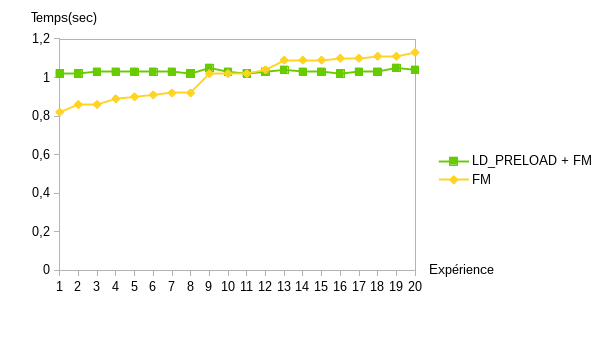
\includegraphics[scale=0.80]{mesures/graph/Temps_FM.png}
    \caption{Temps d'exécution d'une application temporelle en \textit{mediation par traduction d'adresse} avec interception via LD\_PRELOAD et sans interception}
    \label{Temps_FM}
\end{figure}

\subsubsection{Mediation par traduction d'adresse}
Nous allons maintenant voir s'il en est de même pour les deux dernières expériences: Simterpose en \textit{médiation par traduction d'adresse} avec et sans intercpetion via LD\_PRELOAD. On constate ici aussi que le temps d'exécution avec interception via LD\_PRELOAD est plus ou moins constant (environ 1,02 seconde), alors que celui sans interception varie énormément, entre 0,86 et 1,12 secondes. Cela est dû comme précédement à l'utilisation de la bibliothèque VDSO en l'absence d'interception via LD\_PRELOAD. De plus, ici aussi le temps moyen des deux expériences est le même: 1,02 secondes. Dans ce cas, l'interceprtion via LD\_PRELOAD n'a aucun surcoût.

\begin{figure}
  \centering
    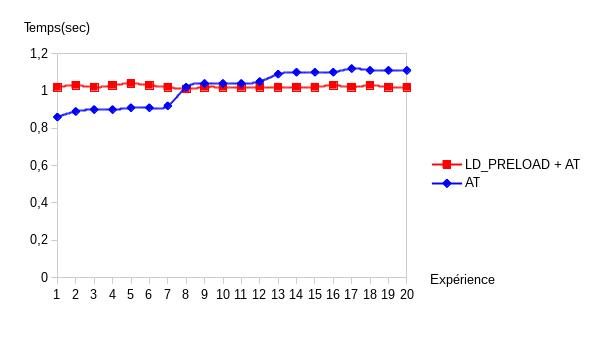
\includegraphics[scale=0.65]{mesures/graph/Temps_AT.jpg}
    \caption{Temps d'exécution d'une application temporelle en \textit{full mediation} avec interception via LD\_PRELOAD et sans interception}
    \label{Temps_AT}
\end{figure}

Ainsi, nous avons pu voir que le surcoût dû à l'interception des fonctions temporelles via LD\_PRELOAD est inexistant en \textit{médiation par traduction d'adresse} et qu'il est négligeable \textit{full mediation} (environ 2\%). On peut donc considérer que nous avons réussi à mettre en place une virtualisation légère qui gère également l'écoulement du temps et qui plus est de façon particulièrement efficace.

\vspace{0.5cm}
